\Inicio{REVIEW}{Potencial terapéutico del uso de adaptógenos en el manejo del estrés y la ansiedad}{Jesús Omar Hampl Chavira, Fernando De La Peña Coutiño, Dioselin Ivanna Méndez Toledo, David Ernesto Vazquez Bernal, Alejandro Sánchez Gaxiola}

\Resumen{El estrés y la ansiedad representan uno de los principales problemas de salud en la población económicamente activa. Los adaptógenos han surgido como una alternativa con potencial terapéutico para mejorar la respuesta del organismo frente al estrés. El objetivo de este estudio fue evaluar el potencial terapéutico del uso de adaptógenos en el manejo del estrés y la ansiedad mediante una revisión sistemática. Se realizó una búsqueda bibliográfica de ensayos clínicos con diseño experimental de doble ciego que evaluaran la reducción del estrés mediante la Escala de Estrés Percibido (PSS) y de niveles de cortisol en suero. Se seleccionaron ocho de estos estudios para el análisis estadístico. Los resultados mostraron un efecto significativo de los adaptógenos en la reducción del estrés percibido (g=1.442, p=0.007), aunque con alta heterogeneidad entre estudios (I$ {2}$=90.04). Asimismo, se observó una reducción significativa en los niveles de cortisol en suero (g=0.509, p=0.009) y heterogeneidad nula (I$ {2}$=0). Esto sugiere que los adaptógenos pueden contribuir a la reducción del estrés y la ansiedad, aunque se requiere mayor investigación con diseños experimentales más uniformes y una mayor diversidad de especies adaptógenas para confirmar su eficacia terapéutica.}{adaptógenos, estrés laboral, ansiedad, cortisol, Escala de Estrés Percibido, meta-análisis}


    \begin{multicols}{2}
    

\section{Introducción}

\subsection{Estrés}

Según la \citet{medlineplus2024}, el estrés es una respuesta física y emocional que se produce cuando una persona enfrenta situaciones que percibe como desafiantes, amenazantes o demandantes. Esta reacción forma parte del mecanismo natural de defensa del organismo y permite responder ante peligros o exigencias del entorno. En pequeñas cantidades, el estrés puede ser positivo, ya que ayuda a mantener el estado de alerta y mejorar el desempeño ante ciertas situaciones, sin embargo, la aparición continua de este provoca la liberación sostenida de hormonas que pueden aumentar el riesgo de desarrollar hipertensión, ansiedad, depresión, trastornos del sueño y fatiga. Además, el estrés laboral ocurre cuando las demandas y presiones del trabajo no corresponden con los conocimientos y habilidades del trabajador, desafiando su capacidad para afrontarlas \citep{who2020}.

Existen dos tipos principales de estrés: el estrés agudo y el estrés crónico. El estrés agudo es de corta duración y aparece ante situaciones inmediatas, como resolver un problema o enfrentar un peligro. Por otro lado, el estrés crónico se mantiene durante semanas o meses y puede estar relacionado con problemas laborales, económicos, familiares o de salud \citep{apa2010}.

Cuando el estrés se prolonga en el tiempo, el cuerpo permanece en estado de alerta constante. Durante esta respuesta, el organismo libera hormonas que aumentan la frecuencia cardíaca, tensan los músculos y mantienen el cerebro más atento. Sin embargo, si esta activación se mantiene de manera continua, puede afectar la salud y aumentar el riesgo de desarrollar problemas como hipertensión, ansiedad, depresión, trastornos del sueño y fatiga. 

De acuerdo con la \citet{medlineplus2024}, el estrés prolongado puede influir negativamente en el bienestar físico y mental, especialmente cuando no se adoptan estrategias adecuadas para su manejo.

\subsection{Estrés laboral}

Según la Organización Mundial de la Salud el estrés laboral se define como la respuesta que pueden presentar las personas cuando las demandas y presiones del trabajo no corresponden con sus conocimientos y habilidades, desafiando su capacidad para afrontarlas. Este fenómeno puede originarse por una organización inadecuada del trabajo, un mal diseño de las tareas, falta de control sobre los procesos laborales, deficiencias en la gestión, condiciones laborales insatisfactorias y escaso apoyo por parte de supervisores o compañeros \citep{maulik2017}.

A nivel global, 40\% de los empleados reportó haber experimentado mucho estrés el día anterior (Gallup, Inc., 2025). En Latinoamérica, alrededor del 43\% de los empleados experimentó mucho estrés el día anterior, con cifras más elevadas en algunos países como Bolivia (55\%), República Dominicana y Costa Rica (51\%) y Ecuador (50\%) (Bloomberg Línea, 2024). México se ha reportado como uno de los países con más altos niveles de estrés laboral del mundo, con 60\% de los trabajadores sufriendo altos niveles de estrés o ansiedad por trabajo en algún momento \citep{atalayar2022}, y 7 de cada 10 mexicanos experimentan efectos significativos de estrés laboral, aunque 80\% de las empresas no tiene estrategias para reducirlo \citep{corresponsables2023}.

De acuerdo con la Universidad Internacional de la Roja (2024), las principales causas del estrés laboral son la sobrecarga y la subcarga de trabajo, condiciones de trabajo deficientes, ambigüedad del rol a desempeñar, rotación constante de personal e incertidumbre por el futuro.

Como resultado de estos factores, el estrés laboral puede generar diversas consecuencias que afectan tanto al trabajador como a la organización. algunas de las principales son un descenso de la productividad, menor calidad de vida, mayor presencia de enfermedades físicas y/o mentales, aparición de depresión y ansiedad, aumento en la incidencia en alcoholismo y otras adicciones, aparición del Síndrome de burnout, problemas familiares y sociales y mayor cantidad de lesiones laborales.

Estos factores influyen directamente en el bienestar emocional y físico de los trabajadores, ya que pueden generar presión constante, desmotivación e inseguridad. Cuando estas situaciones se prolongan, aumentan el agotamiento, disminuyen el rendimiento y afectan tanto la salud individual como el clima organizacional \citep{unir2024}.

\subsection{Adaptógenos}

Los adaptógenos son sustancias naturales, generalmente extractos de plantas, hierbas u hongos. que se ha definido como agentes capaces de incrementar la capacidad del organismo para enfrentar el estrés físico, químico o biológico, mejorando la resiliencia y promoviendo la estabilidad fisiológica del cuerpo. Desde su origen, el concepto médico de “adaptógeno” fue introducido por Nikolai Lazarev en la década de 1940 para describir sustancias que incrementan la resistencia inespecífica del organismo frente a estresores \citep{liao2018}.

Según \citet{colino2025}, los adaptógenos tienen diferentes funciones sobre el cuerpo y la mente, el denominador común es que ajustan la respuesta del cuerpo al estrés. Las principales funciones de los adaptógenos son un aumento en la resistencia al estrés, una mejor regulación en la respuesta al estrés, calman el sistema nervioso y ayudan a aliviar el dolor. Como tal, los adaptógenos no eliminan el estrés, actúan como reguladores: equilibran hormonas, fortalecen la resistencia del cuerpo y ayudan al sistema nervioso a mantenerse estable frente a factores estresantes.

\subsection{Marco legal}

Para el uso de adaptógenos como tratamiento de padecimientos como el estrés y la ansiedad son aplicables ciertas normas y leyes que es necesario conocer para realizar un uso controlado de estas sustancias, esto tanto a nivel nacional como internacional.

A nivel nacional, las normas aplicables son la NOM-051-SCFI/SSA1-2010, que determina las especificaciones generales de etiquetado para alimentos y bebidas no alcohólicas preenvasados, así como la declaración de su información comercial y sanitaria; la NOM-120-SSA1-1994, que establece los bienes y servicios. Prácticas de higiene y sanidad para el proceso de alimentos, bebidas no alcohólicas y alcohólicas; y la NOM-251-SSA1-2009, que indica las prácticas de higiene para el proceso de alimentos, bebidas y suplementos alimenticios.

En materia internacional podemos encontrar también normas que son aplicables al uso de adaptógenos. Se pueden recuperar la ISO 22000, que determina los sistemas de gestión necesarios para asegurar la inocuidad de los alimentos; la ISO 9001, que indica los requisitos para todo sistema de gestión de la calidad; y la ISO 13485, que establece reglamentaciones hacia dispositivos médicos. También debe mencionarse el Codex Alimentarius, que es aplicable para el aspecto del etiquetado, del uso de aditivos, la presencia de contaminantes (tolerancias) y las prácticas de higiene que se deben tener durante el procesamiento del producto.

\section{Materiales y métodos}

\begin{figure}[H]
    \centering
    \fbox{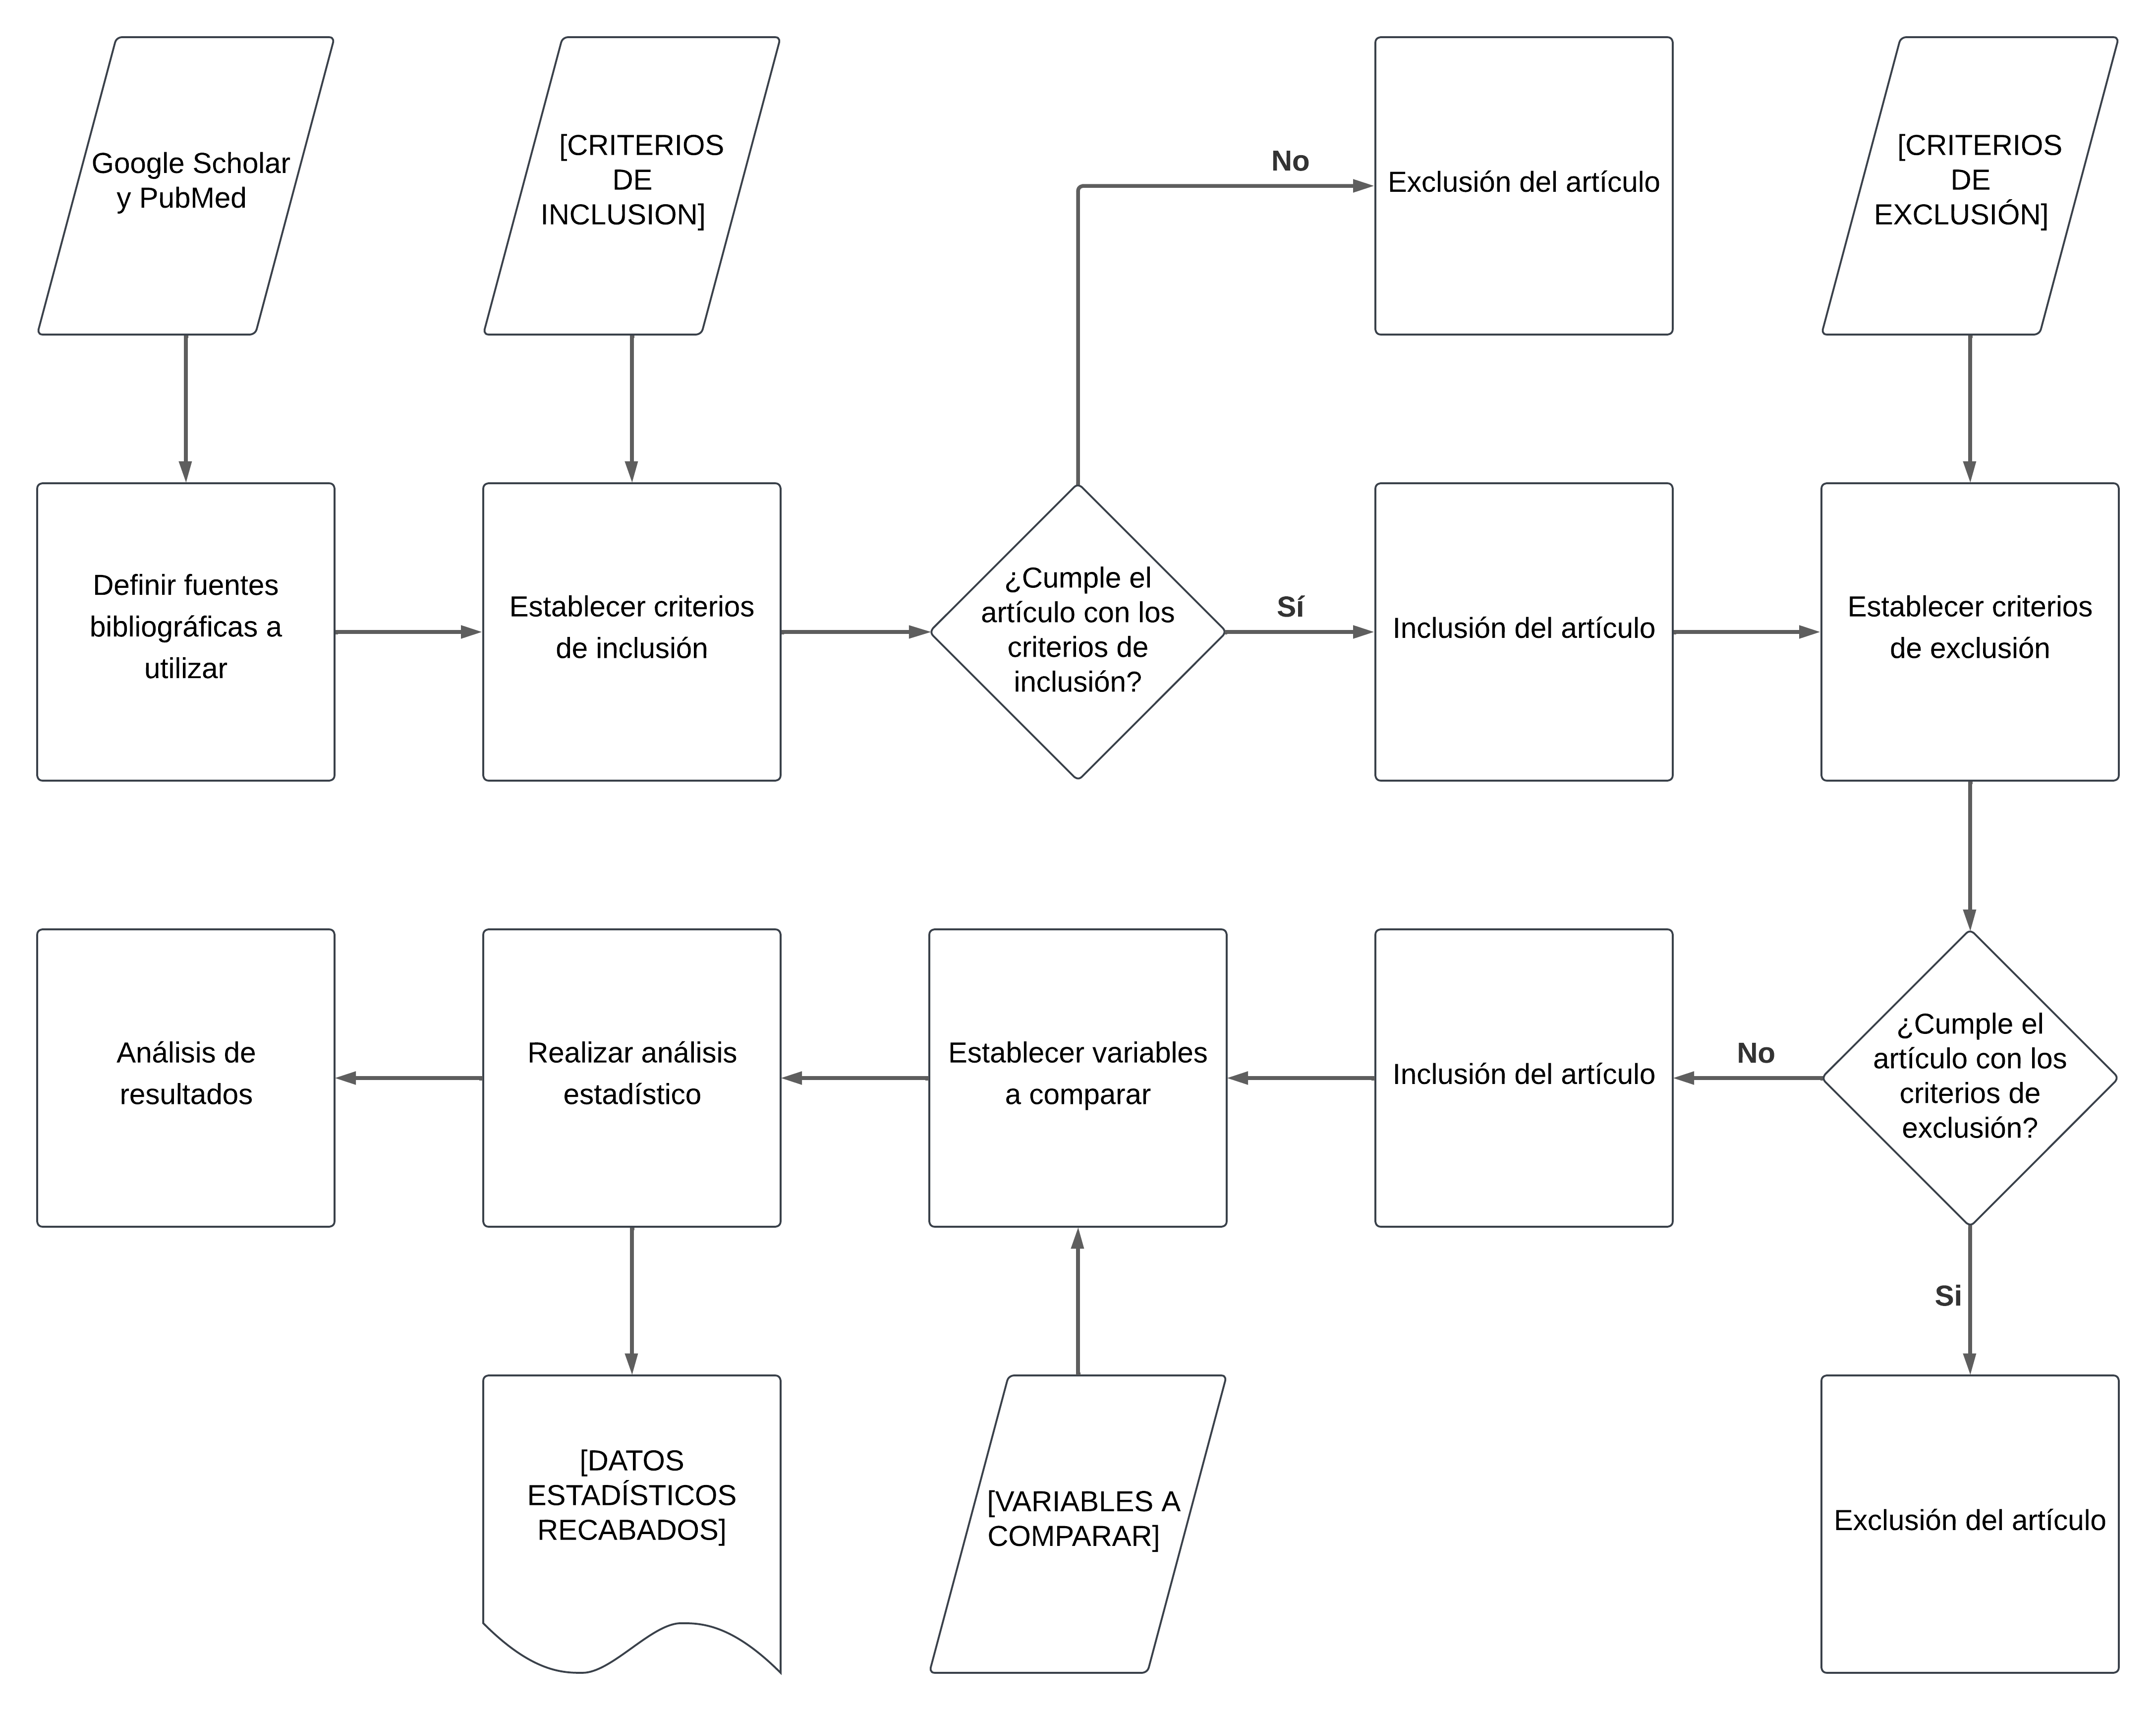
\includegraphics[width=\linewidth]{art_03/Images/Diagrama_Metodología}}
    \caption[Diagrama metodológico]{Metodología de revisión bibliográfica}
    \label{fig:Diagrama_Metodología}
\end{figure}

La presente investigación se desarrolló bajo un enfoque cuantitativo de tipo documental, mediante una revisión sistemática de la literatura científica disponible sobre el uso de hongos adaptógenos en el manejo del estrés y la ansiedad. El propósito fue analizar de manera comparativa la evidencia clínica existente, sin realizar experimentación directa, a partir de estudios previamente publicados en revistas científicas indexadas. El proceso metodológico seguido en la presente investigación se resume en la \autoref{fig:Diagrama_Metodología}.

Se realizó una revisión sistemática con análisis estadístico descriptivo comparativo de ensayos clínicos en humanos. La unidad de análisis no fueron individuos, sino artículos científicos que evaluaran el efecto de plantas y hongos adaptógenos en variables relacionadas con estrés, ansiedad o biomarcadores asociados, como el cortisol. 

\subsection{Búsqueda bibliográfica}

La búsqueda bibliográfica se llevó a cabo en bases de datos científicas reconocidas, tales como PubMed y Google Scholar. Se utilizaron combinaciones de palabras clave en inglés y español, entre ellas: ``adaptogenic mushrooms'', ``Ganoderma lucidum AND stress'', ``Hericium erinaceus AND anxiety'', ``clinical trial AND mushroom AND stress''. Se consideraron artículos publicados entre los años 2016 y 2026, con el fin de incluir evidencia científica reciente y relevante.
La población de estudio estuvo conformada por la totalidad de artículos científicos disponibles en bases de datos indexadas que abordaron el uso de plantas y hongos adaptógenos en el manejo del estrés y la ansiedad en humanos.

\subsubsection{Criterios de inclusión y exclusión}

La muestra estuvo integrada por los estudios que cumplieron con los criterios de inclusión establecidos. Inicialmente se identificó un conjunto amplio de artículos mediante la estrategia de búsqueda; posteriormente, tras la eliminación de duplicados y la aplicación de los criterios de selección, se incluyeron únicamente aquellos estudios que aportaran datos estadísticos cuantificables y pertinentes para el análisis comparativo. Se empleó un muestreo no probabilístico por criterios, seleccionando únicamente los estudios que cumplieran con condiciones específicas previamente definidas. Este tipo de muestreo es adecuado en revisiones sistemáticas, ya que permite delimitar el análisis a investigaciones con rigor metodológico y relevancia directa para el objetivo del estudio.

Los criterios de inclusión fueron ensayos clínicos, uso de diseño experimental de doble ciego y como parámetro de estudio la Escala de Estrés Percibido (PSS por sus siglas en inglés) y los niveles de cortisol. Como criterios de exclusión se establecieron estudios en modelo animales, artículos de revisión y artículos duplicados.

\subsection{Análisis estadístico}

De cada estudio seleccionado se extrajeron las siguientes variables: duración del ensayo, población de los grupos experimentales (con muestra y con placebo), rango de edades de participantes, especie de adaptógeno utilizado, dosis administrada y reducción en los valores de PSS y cortisol en suero sanguíneo. La información fue organizada en una matriz comparativa con el fin de sistematizar los datos y facilitar su análisis.
Se realizó un análisis estadístico descriptivo comparativo de los estudios incluidos. Se calcularon primero las medidas del efecto de los diferentes estudios, primero para los datos midiendo los tests PSS y posteriormente con los datos de cortisol en suero, ambos mediante un diseño de grupos independientes, con medidas cuantitativas y un tamaño de efecto de diferencia de medias estandarizadas (SMD por sus siglas en inglés) con corrección de Hedge (g de Hegde). Posteriormente se realizaron dos meta-análisis. Para el primero, que analiza los resultados de las pruebas de PSS, se utilizó el modelo de efectos aleatorios (REML por sus siglas en inglés), añadiendo como covariables los días de duración de los ensayos, las poblaciones de estos y las dosis administradas, así como un gráfico de embudo con sus respectivos tests de asimetría mediante metarregresión y mediante test de Egger, esto para verificar cuánto afectan las covariables definidas a los resultados de las pruebas PSS. En el segundo meta-análisis se analizó la reducción en los niveles de cortisol de los sujetos, usando de igual manera el modelo REML y usando como covariables los días de duración del ensayo y las dosis administradas. Por el tamaño de la muestra de este segundo meta-análisis, no se realizó gráfico de embudo.

\section{Resultados}

Se identificaron 13 artículos que cumplieron con los criterios de inclusión, siendo todos estos ensayos clínicos en humanos que utilizaban la escala PSS para analizar el efecto de adaptógenos en el manejo del estrés. Puesto que 10 de los artículos administraban el adaptógeno en polvo mediante cápsulas, se excluyeron 3 artículos cuyas dosis consistían en infusiones de mezclas de hongos cuyas formulaciones variaban ligeramente entre estudios. Otro artículo fue excluido por utilizar mezclas de adaptógenos en lugar de un solo organismo al igual que el resto de artículos. Por último, un artículo fue excluido por no declarar la composición exacta de la dosis administrada. La revisión fue realizada a partir de los 8 artículos restantes (\autoref{tab:matriz_comparativa_ensayos_clínicos}).

De los 8 artículos revisados, 7 de ellos corresponden a análisis con la planta \textit{Withania somnifera}, mientras que 1 utilizó la planta \textit{Panax ginseng}.

El meta-análisis sobre el efecto de los adaptógenos sobre el estrés percibido (PSS) mostró un efecto significativo en la reducción de tal parámetro (g=1.442, p=0.007), indicando que los adaptógenos pueden llegar a apoyar en la reducción del estrés percibido, sin embargo, se encontró también una alta heterogeneidad entre los resultados de los estudios (I$ {2}$=90.04, p=0.001) (\autoref{tab:meta_análisis_efetos_adaptógenos_PSS}).

\end{multicols}

    \begin{table}[H]

\caption{Matriz comparativa de ensayos clínicos}
\label{tab:matriz_comparativa_ensayos_clínicos}

\begin{threeparttable}

{\small\setstretch{1.35}\rowcolors{3}{White}{Grey}

\begin{tabular}{M{3em}M{5em}M{5em}M{3em}M{4em}M{4em}M{4em}M{4em}M{6em}M{6em}}\hline
    
    \multirow{3}{3em}{\tmultiheader{Días}} & \multirow{3}{5em}{\tmultiheader{Población (M)\tnote{1}}} & \multirow{3}{5em}{\tmultiheader{Población (PLC)\tnote{2}}} & \multirow{3}{3em}{\tmultiheader{Dosis (mg/día)}} & \multicolumn{4}{c}{\tmultiheader{Reducción\tnote{3}}} & \multirow{3}{6em}{\tmultiheader{Adaptógeno}} & \multirow{3}{6em}{\tmultiheader{Referencia}} \\
    & & & & \tmultiheader{PSS (M)} & \tmultiheader{PSS (Plc)} & \tmultiheader{Cortisol (M)} & \tmultiheader{Cortisol (Plc)} & & \\ \hline
    
    84 & 45 & 45 & 125 & 1.05 (0.52) & 0.55 (0.46) & --- & --- & \textit{W. somnifera} & \citep{panossian2018} \\
    76 & 25 & 25 & 500 & --- & --- & --- & --- & \textit{W. somnifera} & \citep{bishop2015} \\
    56 & 25 & 25 & 600 & 3.83 (3.18) & 1.32 (2.1) & --- & --- & \textit{W. somnifera} & Choudhary et al. (2017) \\
    21 & 70 & 72 & 200 & --- & --- & --- & --- & \textit{Panax ginseng} & Dormal et al. (2025) \\
    56 & 24 & 22 & 500 & --- & --- & --- & --- & \textit{W. somnifera} & Pandit et al. (2024) \\
    168 & 45 & 46 & 600 & 5.02 (3.91) & 2.55 (4.2) & --- & --- & \textit{W. somnifera} & Pakhale et al. (2025) \\
    90 & 62 & 63 & 300 & 2.7 (2.31) & 1.63 (3.31) & --- & --- & \textit{W. somnifera} & Gopukumar et al. (2021) \\
    84 & 55 & 56 & 400 & --- & --- & --- & --- & \textit{W. somnifera} & Smith et al. (2023) \\
    \hline
\end{tabular}

}

\begin{tablenotes}\tiny % ex: \tnote{1} ... \item[1]
    \item[1] M = Muestra;
    \item[2] Plc = Placebo;
    \item[3] Reportado en [Reducción (Desviación estándar)]
\end{tablenotes}

\end{threeparttable}
\end{table}

\begin{multicols}{2}

La metarregresión no identificó asociaciones significativas entre las covariables analizadas (días de duración del ensayo, población de estos y dosis administradas) y la disminución del estrés percibido (\autoref{tab:covariables_adaptógenos_PSS}). Por otro lado, los tests de asimetría del gráfico de embudo reflejaron una asimetría significativa.

En el caso del meta-análisis del efecto de los adaptógenos sobre el cortisol en suero sanguíneo, este también mostró un efecto significativo en la reducción de tal parámetro (g=0.509, p=0.009). A diferencia del anterior, este meta-análisis mostró heterogeneidad nula (I$^{2}$=0, p=0.951), indicando una alta concordancia entre estudios (\autoref{tab:meta_análisis_cortisol}).

Así mismo, la metarregresión mostró una correlación significativa entre las covariables analizadas (días de duración del ensayo y dosis administradas) y la reducción de cortisol en suero sanguíneo. Específicamente, la duración del ensayo mostró una relación directa con la reducción de cortisol, mientras que la dosis administrada mostró una relación inversa, pues la reducción en los niveles de cortisol es menor al aumentar la dosis (\autoref{tab:covariables_cortisol}).

    \begin{table}[H]

\caption{Meta-análisis de los efectos de los adaptógenos en el estrés percibido}
\label{tab:meta_análisis_efetos_adaptógenos_PSS}

\begin{threeparttable}

{\small\setstretch{1.35}\rowcolors{1}{Grey}{White}

\begin{tabular}{M{0.35\linewidth}M{0.25\linewidth}M{0.25\linewidth}}\hline

    \theader{} & \theader{Contraste} & \theader{p} \\ \hline
    
    Heterogeneidad de los errores (I$^{2}$) & 90.042 & < 0.001 \\
    Efecto combinado (g) & 1.442 & 0.007 \\

    \hline
\end{tabular}

}

\begin{tablenotes}\tiny % ex: \tnote{1} ... \item[1]
    \item[] 
\end{tablenotes}

\end{threeparttable}
\end{table}
    \begin{table}[H]

\caption{Asociaciones entre covariables de ensayo y el efecto de los adaptógenos en el estrés percibido.}
\label{tab:covariables_adaptógenos_PSS}

\begin{threeparttable}

{\small\setstretch{1.35}\rowcolors{1}{Grey}{White}

\begin{tabular}{M{0.2\linewidth}M{0.1375\linewidth}M{0.1375\linewidth}M{0.1375\linewidth}M{0.1375\linewidth}}\hline
    
    \theader{} & \theader{F} & \theader{gL$_{1}$} & \theader{gL$_{2}$} & \theader{p} \\ \hline

    Días de ensayo & 2.444 & 1 & 4 & 0.193 \\
    Población del ensayo & 4.229 & 1 & 4.000 & 0.109 \\
    Dosis administrada & 2.391 & 1 & 4.000 & 0.197 \\

    \hline
\end{tabular}

}

\begin{tablenotes}\tiny % ex: \tnote{1} ... \item[1]
    \item[] 
\end{tablenotes}

\end{threeparttable}
\end{table}

    \begin{table}[H]

\caption{Meta-análisis de los efectos de los adaptógenos en niveles de cortisol en suero sanguíneo.}
\label{tab:meta_análisis_cortisol}

\begin{threeparttable}

{\small\setstretch{1.35}\rowcolors{1}{Grey}{White}

\begin{tabular}{M{0.35\linewidth}M{0.25\linewidth}M{0.25\linewidth}}\hline
    
    \theader{} & \theader{Contraste} & \theader{p} \\ \hline
    Heterogeneidad de los errores (I$^{2}$) & 0.000 & 0.951 \\
    Efecto combinado (g) & 0.509 & 0.009 \\

    \hline
\end{tabular}

}

\begin{tablenotes}\tiny % ex: \tnote{1} ... \item[1]
    \item[] 
\end{tablenotes}

\end{threeparttable}
\end{table}
    \begin{table}[H]

\caption{Asociaciones entre covariables de ensayo y el efecto de los adaptógenos en niveles de cortisol en suero sanguíneo}
\label{tab:covariables_cortisol}

\begin{threeparttable}

{\centering\small\setstretch{1.35}\rowcolors{1}{Grey}{White}

\begin{tabular}{M{0.2\linewidth}M{0.1375\linewidth}M{0.1375\linewidth}M{0.1375\linewidth}M{0.1375\linewidth}}\hline

    \theader{} & \theader{F} & \theader{gl$_{1}$} & \theader{gL$_{2}$} & \theader{p} \\ \hline
    
    Días de ensayo & 188.5 & 1 & 1.000 & 0.046 \\
    Dosis administrada & 137502.1 & 1 & 1.000 & 0.180 \\

    \hline
\end{tabular}

}

\begin{tablenotes}\tiny % ex: \tnote{1} ... \item[1]
    \item[] 
\end{tablenotes}

\end{threeparttable}
\end{table}

\section{Discusión}

El que la mayoría de estudios encontrados fueran acerca de plantas, sobre todo de \textit{W. somnifera}, refleja una necesidad de diversificar los estudios de adaptógenos hacia una mayor diversidad de especies, sobre todo alrededor de hongos, acerca de los cuales existe una bibliografía limitada y heterogénea, con un diseño experimental poco uniforme \citep{panossian2018}.

Si bien los ensayos con adaptógenos mostraron un efecto significativo en el estrés percibido, estos no terminaron de ser consistentes entre sí, pues el efecto no fue igual en todos los estudios. La falta de asociaciones significativas entre las covariables relacionadas al diseño de los ensayos muestran que no son las diferencias entre los diseños experimentales de los estudios lo que está causando esta heterogeneidad en los resultados. Todo lo anterior, complementado con la alta asimetría reflejada en el gráfico de embudo, indica un posible sesgo de publicación.

En el caso de los niveles de cortisol los resultados son más concluyentes, pues existe una nula heterogeneidad en los resultados, mostrando que los adaptógenos ayudan en la reducción de esta hormona. Los resultados de la metarregresión indican que el extender el uso de adaptógenos ayuda a mejorar la reducción de cortisol en suero sanguíneo. A diferencia de la variable del tiempo, la dosis administrada muestra una relación inversa, lo que podría ser indicador de efecto hormesis, sin embargo, es necesaria una muestra más grande de estudios al respecto para confirmar este efecto \citep{wachtelgalor2011}.

\section{Conclusión}

Si bien las sustancias adaptógenas reportan tener un impacto real y significativo en la prevención del estrés y de la ansiedad, los estudios que evalúan tales aspectos utilizan una baja variedad de organismos para el análisis, así como metodologías muy variables entre sí. Es necesario pues una estandarización de las metodologías así como una diversificación en los organismos a evaluar, esto para poder contar con una conocimiento más amplio y completo del potencial terapéutico de estos en el manejo de los padecimientos mentales mencionados.

% ------------------------------------------------------\%

\bibliographystyle{apalike-ejor}
\bibliography{art_03/bib}

\end{multicols}